This section describes the actual plugin, ie.~which tasks have been implemented, and the features and usage of the plugin.
Protege was developed in Java, it can easily be extended in the form of \emph{plugins} which are typically Java Archive (.jar) files
stored in the Protege \texttt{plugin} directory. The most common form of a Protege plugin is a \emph{view plugin}, which implements a single view for a specific area of an ontology (e.g. classes, individuals, object properties, \dots).
%Florian: Protege completely was programmed in Java, therefore all plugins also are programmed in Java. Since Protege was developed very modular, it is quite easy to create simply plugins and integrate them into Protege. 
%Florian: All Protege plugins are so called jar-Files (Java Archive), and contains the compiled source code and all needed libraries. The most common form of a Protege plugin is a view plugin, which implements a single view for a specific area of an ontology (e.g. classes, individuals, object properties, ...)

% installation / SETUP 
\textbf{Installation and setup.}
The plugin is available at \url{TODO -- add link once uploaded to Protege}, includes detailed documentation about the tasks and
the usage of the plugin. TODO (if necessary) documentation is accessible at ..
To use the plugin you need to your uComp-API key\footnote{Request a key from the uComp team, see \url{http://soc.ecoresearch.net/facebook/election2008/ucomp-quiz-beta/api/v1/documentation/}} in a file named \texttt{ucomp\_api\_key.txt} in folder \texttt{.Protege}.


%Florian: The CF key has to be associated with the uComp-API key, therefore it has to be communicated to the uComp-API team (see http://soc.ecoresearch.net/facebook/election2008/ucomp-quiz-beta/api/v1/documentation/)
%Florian: The uComp-API key itself must be put into a textfile named "ucomp_api_key.txt" at the users home directory, in the folder ".Protege" (which is created by Protege during installation on both Windows and Linux plattforms) 

%Florian: all information about the task is stored (depends on the kind of task): domain, validation of whole subtree going on?, additional information, sent to crowdflower or ucomp-quiz, ucomp-api job-id, ...

% give an example SCREEENSHOT with a quick introduction 
\begin{figure*}[htb]
\centering
{\centering \resizebox*{1.0\textwidth}{!}{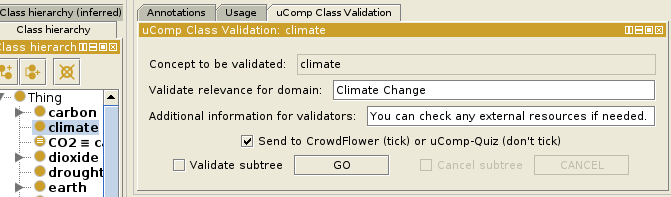
\includegraphics{images/c_rel_check_start.png}}}
 \caption{\label{fig:screen_cr}Screenshot showing the interface for validating a concept.}
\end{figure*}

Figure~\ref{fig:screen_cr} shows the basic interface for the domain relevance task, the other tasks
have similar interface.
Initially, the user adds the new view in the Protege window. The plugin interface contains
task specific information (eg. the concept selected by the user for validation),
generic information such as the \emph{domain} of the ontology and \emph{additional information} (see below),
and a \texttt{GO} button start the validation process. \\


% The common PROCESS (in short)
\textbf{Usage.} The process itself is similar for all types of evaluations:
\begin{enumerate}
\item Add the corresponding view to the user interface via the \emph{Window $\rightarrow{}$ Views} menu. The ontology engineer
selects the part of the ontology to verify (eg. the \emph{classes}), and adds the corresponding uComp HC validation frame to the user interface. 
\item The user selects which part of the ontology should be verified (eg. a specific class or all classes in the ontology).
\item The user can provide additional information and options in the plugin view and then starts the evaluation.
\item A requested is sent to the uComp API.
\item Depending on user settings, the uComp API delegates the job to a GWAP or to CrowdFlower.
\item As soon as available, the plugin presents the results to the user and saves them in the ontology.
\item The user can always cancel (pause) the validation process.
\item Depending on the result, the user will perform further actions such as deleting parts of the ontology which have been validated as non-relevant.
\end{enumerate}

%After enough HC users given their input on the task, the results are sent back to the plugin, which then displays them to the Protégé user. 
%Depending on the result, the user can perform further actions like deleting negatively validated parts of the ontology.


% PERSISTENCE 
All data collected by the plugin which should be persistent is stored in the ontology in \texttt{rdfs:comment} fields,
for example information about the domain, the job ID, and results from the game.


% COMMON FIELDS in the UI: domain and additional information & validate subtree
\textbf{The User Interface}
What is common among all tasks handled by the plugin, is the selection of a \emph{domain} and that the user can provide
additional information about the task. The domain is simply the field of knowledge which the ontology covers. If entered
once, the domain will be stored in the ontology (as \texttt{rdfs:comment}) and be pre-filled subsequently, but it can also be changed at any time.
For every task, the plugin contains a predefined task description (typically including examples) which is presented to the HC user.
If the ontology engineer wants to extend this task description, he or she can provide more guidelines in the field \emph{additional information}.
In many cases the user of the plugin wants to verify not only a single class, but a part of the ontology, or even the whole ontology.
This can be achieved with the \emph{Validate subtree} option. If the option is selected, the current concept and all its subconcepts 
are verified (recursively). The verify the entire ontology, the user just starts from the uppermost class (\emph{Thing}).
In the remainder of the section we give some details about the parts of the plugin used in the evaluation (see Section~\ref{sec:eval}),
ie.~verification of domain relevance and of relation correctness.
%Florian: domain will be stored as rdfs:comment in the head of the ontology

% T1. Verification of Domain Relevance.  Is a concept/instance relevant for a domain?
% T2. Verification of Relation Correctness. Does a certain relation between two ontology entities hold? These could be a set of generic relations (sameAs, subClassOf, instanceOf), but also arbitrary named relations to be specified by the ontology engineer. The crowd here would have to vote (yes/no) for a given triple (Subject - Relation - Object). This task is the focus of [1].


% TASKs
\textbf{Task 1 - Verification of Domain Relevance.}
Verification of domain relevance of a class (called ``uComp Class Validation'' in the plugin) helps to decide if a concept (class) is relevant for a domain. 
First, the ontology engineer adds the corresponding view (\emph{Window} $\rightarrow{}$ \emph{Views} $\rightarrow{}$ \emph{Class Views} $\rightarrow{}$ \emph{uComp Class Validation}) to the UI.
This is the simplest type of validation task, so the process is very much in line with the \emph{usage} described above.
Figure~\ref{fig:screen_cr} shows the UI for the class ``fracking'' before initiating the verification. 

\begin{figure*}[htb]
\centering
{\centering \resizebox*{1.00\textwidth}{!}{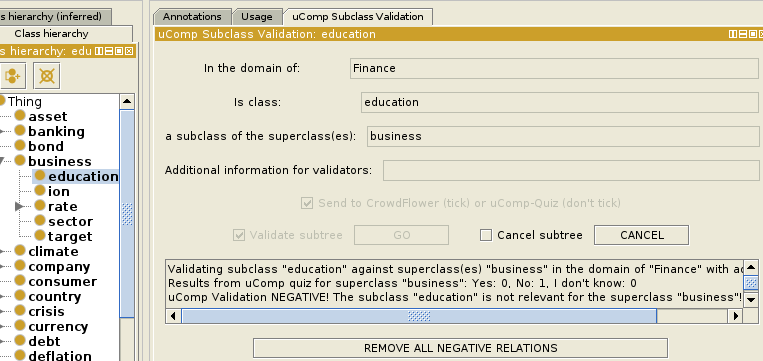
\includegraphics{images/sc_subclass_val.png}}}
 \caption{\label{fig:screen_sub}Screenshot showing the interface for subClassOf relation validation, including the display of results}.
\end{figure*}


\textbf{Task 2 - Verification of Relation Correctness.}
The second task is the verification of relation correctness, more precisely the verfication of IS-A (subClassOf) relations between classes.
The corresponding view is named \emph{Class Views} $\rightarrow{}$ \emph{uComp SubClass Validation}. When selecting a class in Protege,
the plugin automatically detects its superclasses (if any) and fills the boxes in the plugin UI.
As soon as results are available these are presented in the UI, as shown in Figure~\ref{fig:screen_sub}. The screenshot gives an example
wit one evaluator, who rated the \emph{IS-A} relation between ``education'' and ``business'' as invalid. As the majority of ratings is negative,
a button to remove the relation is displayed.

\textbf{Task 3 - 5.}
The uComp Protege plugin also supports 3 other tasks, which we will cover only briefly, as they are not part of the user evaluation in
Section~\ref{sec:eval}. Task 3 is the verfication of \emph{instanceOf} relations between an individual and a class, i.e.~the crowd helps
to verify if a given \emph{instanceOf} is valid. Task 4 is concerned with validating \emph{domain} and \emph{range} of properties, which
results in two separate sub-tasks (domain, range). And finally, we implemented a Protege view component that collects suggestions for 
labelling unlabeled relations from a set of given properties (relations).
